\section{Proces rejestrowania i przetwarzania wielkości analogowych w czasie rzeczywistym}

Zadaniem tego procesu jest odczyt wartości analogowych, które następnie zostają przetwarzanie wewnątrz sterownika PLC. Odczytywane zostają wartości odległości zmierzone za pomocą czujników ultradźwiękowych. Sterownik dokonuje obliczeń, mających na celu obliczenie rzeczywistych wartości odległości. Przetworzone pomiary zostają zapisane do bloku danych służącego jako bufor. W przypadku jego przepełnienia stare wartości zostają nadpisane. Dodatkowo z aktualnie znajdujących się w buforze pomiarów obliczane są wartości minimalne, maksymalne oraz średnie.

\subsection{Moduł we/wy analogowych Simatic SM 334}
Odczyt danych analogowych wykonywany poprzez moduł wejść/wyjść analogowych Simatic SM 334.
\begin{figure}[h]
\centering
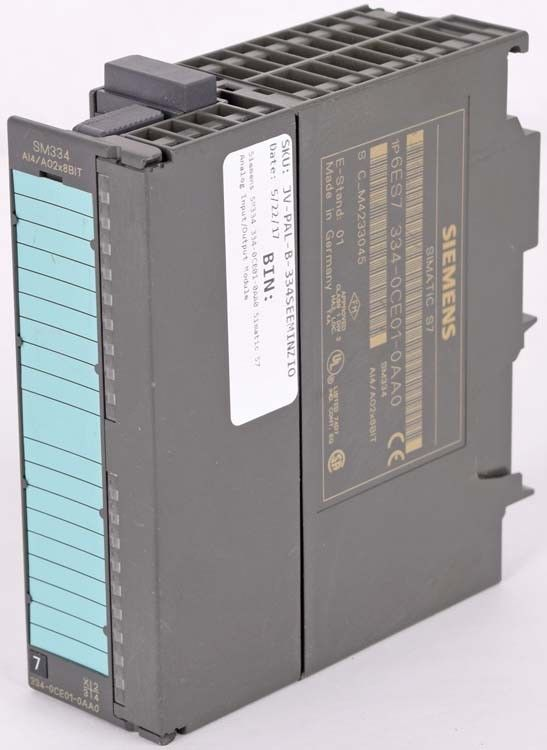
\includegraphics[scale=1.2]{Zdjecia/Stanowiska/2_Czujniki_Odleglosci/sm334.jpg}
\caption{Moduł SM334}
\end{figure}

\newpage

Moduł ten pozwala na odczyt wartości analogowych mogących być wartością napięcia, rezystancji bądź temperatury. Posiada on 4 kanały wejściowe pozwalające na następujące kombinacje podłączeń:
\begin{table}[h]
\centering
 \begin{tabular}{||c | c ||} 
 \hline
 Jednostka & Zakres  \\ 
 \hline\hline
 Kanały 0 i 1 
 & \tabitem 2x temperatura  \\
 & \tabitem 2x rezystancja  \\
 \hline
 Kanały 2 i 3
 & \tabitem 2x napięcie \\
 & \tabitem 2x temperatura \\
 & \tabitem 2x rezystancja \\
 & \tabitem 1x temperatura, 1x napięcie \\
 & \tabitem 1x rezystancja, 1x napięcie \\
 \hline
\end{tabular}
\caption{Podłączenie kanałów wejściowych modułu SM334}
\end{table}

Ponadto moduł posiada 2 wyjścia napięciowe o maksymalnym napięciu równym 10 V.

Kanał wejściowy poddaje odczytaną wartość konwersji analogowo-cyfrowej po czym zapisuje ją do rejestru 16-bitowego. Programistyczny dostęp do tych rejestrów dostępny jest poprzez wejścia peryferyjne.

Zakres wartości wejściowych prezentuje poniższa tabela:

\begin{table}[h]
\centering
 \begin{tabular}{||c | c ||} 
 \hline
 Jednostka & Zakres  \\ [0.5ex] 
 \hline\hline
 Napięcie & 0 - 10 [V]  \\ 
 \hline
 Rezystancja & 0 - 10 [$k\Omega$]  \\
 \hline
 Temperatura & -120 - 130 [°C]  \\
 \hline
\end{tabular}
\caption{Zakres wartości wejściowych modułu SM334}
\end{table}

Przy tym procesie wykorzystane zostały jedynie 2 kanały wejściowe (2 i 3) jako wejścia napięciowe. Wartości liczbowe po konwersji analogowo-cyfrowej zostały przedstawione w poniższej tabeli:
\begin{table}[h]
\centering
 \begin{tabular}{||c | c ||} 
 \hline
 Wartość napięcia [V] & Wartość liczbowa  \\ [0.5ex] 
 \hline\hline
 > 11.7589 & 32767  \\ 
 \hline
 11.7589 & 32767 \\
 . & . \\
 . & . \\
 10.0004 & 27649\\
 \hline
 10.0000 & 27648\\
 . & . \\
 . & . \\
 7.50000 & 20736\\
 . & . \\
 . & . \\
 0 & 0 \\
 \hline
\end{tabular}
\caption{Przetworzone wartości napięciowe wejścia modułu SM334}
\label{tab:2_wartoscio_napiecia}
\end{table}
